\begin{frame}{Turning ideas into language \parencite{bock1994}}

\begin{minipage}[t]{.475\textwidth}
\begin{small}
\begin{itemize}
	\item Unordered message units
	\item Output has linear order
	\item Linearisation via pragmatic, lexical and / or syntactic factors 
\end{itemize}
\end{small}
\end{minipage}

\begin{backgroundblock}{60mm}{20mm}	
	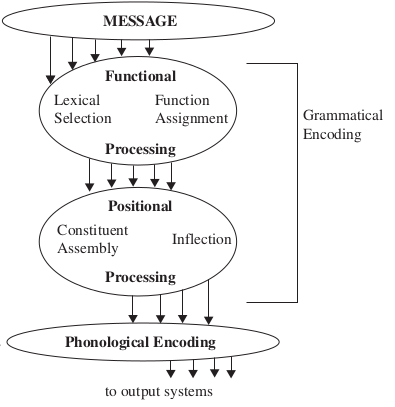
\includegraphics[scale=.45]{gfx/BLmodel.png}
\end{backgroundblock}

\end{frame}

\begin{frame}
	\begin{Large}
		\begin{center}
			\textit{To what extent does syntax affect the linearisation of the output before production onset?}
		\end{center}
	\end{Large}
\end{frame}


\begin{frame}{\only<1,5,10-13>{Syntax in language production \parencite{bock2014syntactically}}}

% P 25 in Bock and Ferreira 2014: Paul (1886/190) and Wundt (1912)
% Paul: incremental lexical view
% Wundt: aboutness relations at the core
% Kuchinski relational vs non-relational 

\only<1,5,10-13>{
\begin{small}
	\begin{enumerate}
	\item \uncover<1->{Syntax is emergent property of lexically-driven planning}
	\item \uncover<5->{Syntax is generated from message representation}
	\begin{itemize}
		\item[a.] \uncover<10->{\textbf{Deterministic:} syntax determines size of planning unit}
		\item[b.] \uncover<11->{\textbf{Non-deterministic:} multiple candidate structures   \parencite{kempen1987incremental}}		
	\end{itemize}
	\item \uncover<12->{Both routes (relational and non-relational) are available \parencite[at the message level; see][]{konopka2014priming}.}
	\end{enumerate}
\end{small}

\vspace{1cm}
\begin{center}
	\uncover<13->{\textit{Consider the following evidence for possibility (2a).}}
\end{center}
}

\begin{backgroundblock}{10mm}{10mm}	
	\only<2,3,4>{
	\begin{tikzpicture}
		\node[anchor=north west,rectangle, draw, thick, rounded corners, draw=black, inner sep=3.5pt] (screen) at (0,0) {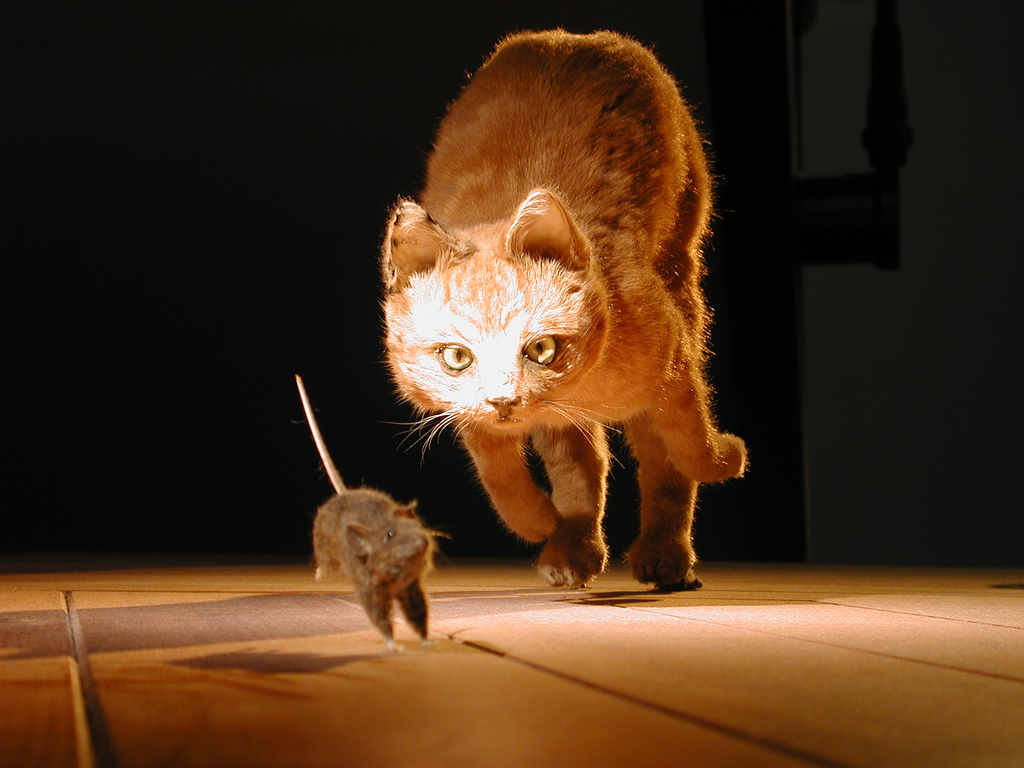
\includegraphics[scale=.1]{gfx/cat2.jpg}};
		
		%% CHUNK 1
		\only<2->{\node[below left = 1cm of screen, rectangle, draw, fill=gray!20!white] (message) {Message};}
		\only<2->{\node[below right = .25cm and 0cm of message, rectangle, draw, fill=gray!40!white, color=gray!40!white] (message2) {Message};}
		\only<2->{\draw[red!60!black, thick] (2.1,-1.2) circle (1cm);}
		\only<2->{\draw[->, thick] (0.9,-1.7) -- (message);}
		\only<2->{\node[below = .25cm of message2, rectangle, draw] (lemma) {CAT};}
		\only<2->{\draw[->, dashed, thick, to path={|- (\tikztotarget)}] (message) edge (message2);}
		
		%% CHUNK 2
		\only<3->{\node[right = .25cm of message, rectangle, draw, fill=gray!20!white, color=gray!20!white] (messageU2) {Message};}	
		\only<3->{\draw[->, thick] (1.2,-2) -- (messageU2);}
		\only<3->{\node[right = .25cm of message2, rectangle, draw, fill=gray!40!white, color=gray!40!white] (messageL2) {Message};}
		\only<3->{\draw[->, dashed, thick, to path={|- (\tikztotarget)}] (messageU2) edge (messageL2);}
		\only<3->{\node[below = .25cm of messageL2, rectangle, draw] (lemma2) {CHASING};}
		
		%% CHUNK 3
		\only<4->{\node[right = .25cm of messageU2, rectangle, draw, fill=gray!20!white, color=gray!20!white] (messageU3) {Message};}	
		\only<4->{\draw[->, thick] (1.5,-2) -- (messageU3);}
		\only<4->{\node[right = .25cm of messageL2, rectangle, draw, fill=gray!40!white, color=gray!40!white] (messageL3) {Message};}
		\only<4->{\draw[->, dashed, thick, to path={|- (\tikztotarget)}] (messageU3) edge (messageL3);}
		\only<4->{\node[below = .25cm of messageL3, rectangle, draw] (lemma3) {RAT};}
		
		
	\end{tikzpicture}
	}
	\only<6-9>{
	\begin{tikzpicture}
		\node[anchor=north west,rectangle, draw, thick, rounded corners, draw=black, inner sep=3.5pt] (screen) at (0,0) {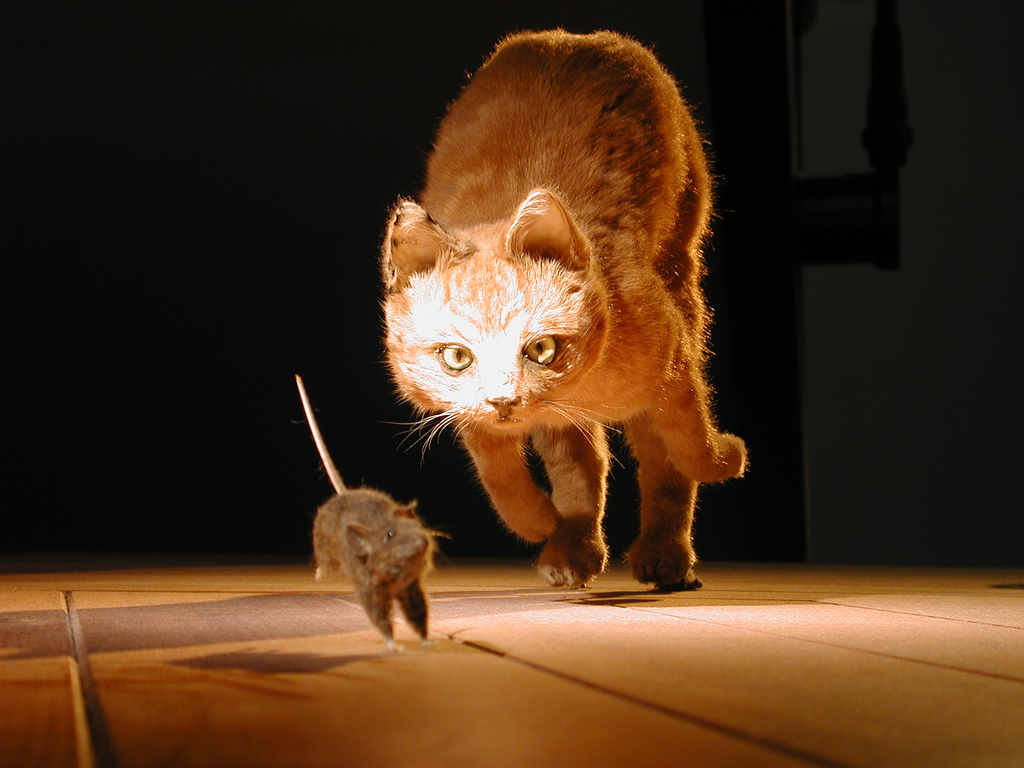
\includegraphics[scale=.1]{gfx/cat2.jpg}};
		\only<6->{\node[below = .5cm of screen, rectangle, draw, fill=gray!20!white] (message) {Message};}
		\only<6->{\draw[->, thick] (1.95,-2.5) -- (message);}
		\only<7->{\draw[->, dashed, thick, to path={|- (\tikztotarget)}] (message) edge (3.5,-4.5);}
		
	\end{tikzpicture}
	}
\end{backgroundblock}

\only<2>{
	\begin{backgroundblock}{33mm}{73mm}	
		\begin{tikzpicture}[level distance=25pt]
			\Tree [.NP ]
			
		\end{tikzpicture}
		
	\end{backgroundblock}
}

\only<3>{
	\begin{backgroundblock}{35mm}{73mm}	
		\begin{tikzpicture}[level 1/.style={level distance=5pt},
			level 2/.style={level distance=25pt}]
			\Tree [ [.NP ] [.VP V ] ]
			
		\end{tikzpicture}
		
	\end{backgroundblock}
}

\only<4>{
	\begin{backgroundblock}{35mm}{73mm}	
		\begin{tikzpicture}[level 1/.style={level distance=5pt},
			level 2/.style={level distance=25pt}]
			\Tree [ [.NP ] [.VP V NP ] ] ]
			
		\end{tikzpicture}
		
	\end{backgroundblock}
}

	\begin{backgroundblock}{40mm}{55mm}	
		\only<7>{
		\begin{tikzpicture}[level 1/.style={level distance=15pt},
			level 2/.style={level distance=25pt}]
			\Tree [ [.NP  \edge[color=white]; \node[draw]{CAT}; ] [.VP \edge[dashed, color = gray!60!white]; {\color{gray!50!white}V} \edge[dashed, color = gray!60!white]; {\color{gray!50!white}NP} ] ] ]
			
		\end{tikzpicture}
	}	
	\only<8>{
	\begin{tikzpicture}[level 1/.style={level distance=15pt, sibling distance=1pt},
		level 2/.style={level distance=25pt}]
		\Tree [ \edge[dashed, color = gray!60!white];
				[.{\color{gray!50!white}NP} ]
					[.VP [.V \edge[color=white]; \node[draw]{CHASE}; ] {\color{gray!50!white}NP} 
					] 
				] 
		
	\end{tikzpicture}
	}	
	\only<9>{
	\begin{tikzpicture}[level 1/.style={level distance=20pt, sibling distance=20pt},
		level 2/.style={level distance=25pt}]
		\Tree [ \edge[dashed, color = gray!60!white];
				[.{\color{gray!50!white}NP} ] \edge[dashed, color = gray!60!white];
					[.{\color{gray!50!white}VP} \edge[dashed, color = gray!60!white]; {\color{gray!50!white}V} 
					 [.NP \edge[color=white]; \node[draw]{RAT}; ]
				] 
			] 
		
	\end{tikzpicture}
	}	
	\end{backgroundblock}




\end{frame}



\begin{frame}%{Image-description task}
	
	\only<1>{
		\begin{flushleft}
			\vspace{4cm}
			\Huge{\textbf{+}}
		\end{flushleft}
	}	
	
	\only<2>{
		\begin{backgroundblock}{20mm}{37mm}		
			
\includegraphics[scale=.35]{gfx/peter2}
		\end{backgroundblock}
		
		\begin{backgroundblock}{55mm}{36mm}		
			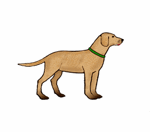
\includegraphics[scale=.4]{gfx/073} 
		\end{backgroundblock}
		
		\begin{backgroundblock}{90mm}{37mm}		
			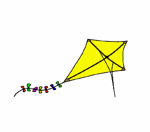
\includegraphics[scale=.4]{gfx/129}
		\end{backgroundblock}
	}
	
	\only<3>{
		\begin{backgroundblock}{20mm}{23mm}		
			
\includegraphics[scale=.35]{gfx/peter2}
		\end{backgroundblock}
		
		\begin{backgroundblock}{55mm}{22mm}		
			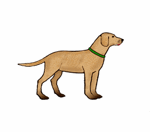
\includegraphics[scale=.4]{gfx/073} 
		\end{backgroundblock}
		
		\begin{backgroundblock}{90mm}{52mm}		
			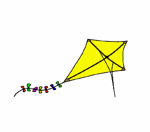
\includegraphics[scale=.4]{gfx/129}
		\end{backgroundblock}
	}
	
	
	\only<4>{
		\begin{center}
			{\huge\textit{The boy and the dog moved above the kite.}}
		\end{center}
	}
	
	
	
\end{frame}


%\blfootnote{\parencite{ martin2014working,martin2010planning, roeser2019advance, smi99, wag10,hardy2019age,hardy2020healthy,ferreira1991effects,levelt1981lexical,wheeldon2013,smith2001,konopka2012planning}}
\begin{frame}
	
	\newcommand{\ImageWidth}{11cm}
	\begin{tikzpicture}
		% draw horizontal line   
		\draw[thick, -Triangle] (0,-1) -- (\ImageWidth,-1) node[font=\scriptsize, below left=3pt and -8pt]{Time (in msecs)};
		
		\node[inner sep=0pt] (stim) at (1.5,-.1) 
		{\fcolorbox{black}{white}{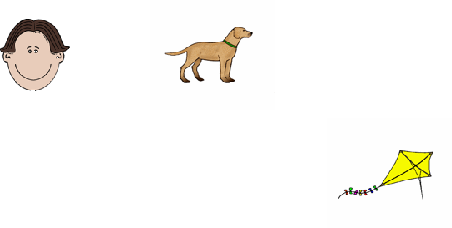
\includegraphics[scale=.351]{gfx/method/build/screen-3}}};
		
		\node[inner sep=0pt, visible on=<2->, right = 3cm of stim] (voice) 
		{
\includegraphics[scale=.2]{speech.jpeg}};
		
		% draw vertical lines
		\foreach \x in {0,1,...,8}
		    	\draw (\x cm,-1) -- (\x cm,-1.2);
    	
		\foreach \x/\descr in {0/0,1/200,2/400,3/600,4/700,5/800,6/900,7/1000,8/1200}
				\node[font=\scriptsize, text height=1.75ex, text depth=.5ex] at (\x,-1.4) {$\descr$};
		

		\draw[-Triangle,dashed,red!60!black,line width=2pt,visible on=<3->] (0,-2) -- +(8,0);
		
		% braces
		\draw [thick,decorate, color = white, visible on=<3->] (5,-2.15) -- +(-1,0)
		node [black,midway,below=4pt] {Onset latency};
		
		\draw[thick, dashed, visible on=<2->](0,-3) -- (0,.7) 
		node[font=\scriptsize] at (1,-3) {Stimulus onset};
		
		\draw[thick, dashed, visible on=<2->](8,-3) -- (8,.7) 
		node[font=\scriptsize] at (7.1,-3) {Voice onset};
		
	\end{tikzpicture}
	\vfill
	\begin{itemize}
		\item[1.] \uncover<2->{\textbf{The boy and the dog} moved above the kite.}
		\item[2.] \uncover<4->{\textbf{The boy} moved above the dog and the kite.}		
	\end{itemize}
	

\end{frame}

\begin{frame}
	
	\newcommand{\ImageWidth}{11cm}
	\begin{tikzpicture}

% draw horizontal line   
\draw[thick, -Triangle] (0,-1) -- (\ImageWidth,-1) node[font=\scriptsize, below left=3pt and -8pt]{Time (in msecs)};

\node[inner sep=0pt] (stim) at (1.5,-.1) 
{\fcolorbox{black}{white}{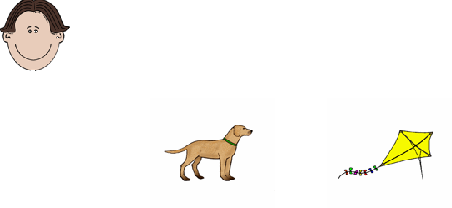
\includegraphics[scale=.351]{gfx/method/build/screen-4}}};

\node[inner sep=0pt, right = 2cm of stim] (voice) 
{
\includegraphics[scale=.2]{speech.jpeg}};

% draw vertical lines
\foreach \x in {0,1,...,8}
\draw (\x cm,-1) -- (\x cm,-1.2);

\foreach \x/\descr in {0/0,1/200,2/400,3/600,4/700,5/800,6/900,7/1000,8/1200}
\node[font=\scriptsize, text height=1.75ex, text depth=.5ex] at (\x,-1.4) {$\descr$};

\draw[-Triangle,dashed,red!60!black,line width=2pt] (0,-2) -- +(7,0);

% braces
\draw [thick,decorate, color = white] (4,-2.15) -- +(-1,0)
node [black,midway,below=4pt] {Onset latency};

\draw[thick, dashed](0,-3) -- (0,.7) 
node[font=\scriptsize] at (1,-3) {Stimulus onset};

\draw[thick, dashed](7,-3) -- (7,.7) 
node[font=\scriptsize] at (6.1,-3) {Voice onset};

		
	\end{tikzpicture}
	\vfill
	\begin{itemize}
		\item[1.] \uncover<1->{\textbf{The boy and the dog} moved above the kite.}
		\item[2.] \uncover<1->{\textbf{The boy} moved above the dog and the kite.}
	\end{itemize}
	
	
\end{frame}


%\begin{frame}{Planning scope in sentence production\blfootnote{\shortciteA<e.g.>{ martin2014working, roeser2018advance, smi99}} }

\begin{frame}{Preplanning is guided by syntax}

\begin{itemize}
		\item Frequently reproduced systematic slowdown for conjoined NPs \parencite[e.g.][]{martin2014working,smi99,wag10,wheeldon2013}.
		\item ``Phrase as default planning scope'' \parencite{martin2010planning}
		\item NP syntax must be planned before onset; hence determines planning scope.
%		\item Deterministic syntax-driven production model (as implied by LMM, ANOVA). 
%		\item Lexical scope is smaller \parencite{gri01} and flexible \parencite{wheeldon2013}.
\end{itemize}

\end{frame}


\begin{comment}
\begin{frame}{Advance planning involves syntax}
\begin{itemize}
	\item Subordination vs coordination with conflicting results \parencite{not07, all07}.
	\begin{itemize}
		\item[2a.] The A with the B is \dots
		\item[2b.] The A and the B are \dots
	\end{itemize}		
	\item Syntactic proximity \parencite{lee13}.
	\begin{itemize}
		\item[3a.] Click on [[the fork of the king] below the apple]
		\item[3b.] Click on [the fork of [the king below the apple]]
	\end{itemize}
	\item Lexical scope is flexible \parencite{wheeldon2013}.
\end{itemize}
\end{frame}
\end{comment}


% Under what circumstances would it be optional to plan phrase syntax or not
% Alternative: syntax planning is non-deterministic
% a. a syntactic route is available as well as a lexical route
% b. a lexical-guided production system can in in principle prepare larger chunks before utterance onset for non-syntactic reasons (distance between nouns; visual grouping).


\begin{frame}{Alternative hypothesis}

\begin{itemize}
	\item \textbf{Preplanning beyond the first noun is more likely but not obligated by the phrase syntax} because, for example, \dots 
	\item[1.] \uncover<2->{Fluency requires preplanning of B in \textit{The A and the B moved \dots} when there isn't enough time to plan B in parallel to articulation \parencite{all07,griffin2003reversed}.}
	\item[2.] \uncover<3->{Correction of incorrectly activated candidate syntax.}
	\item[3.] \uncover<4->{Relational message-level route activated syntactic route.}
\end{itemize}

\end{frame}


